
%%%%%%%%%%%%%%%%%%%%%%%%%%%%%%%%%%%%%%%%%%%%%%%%%%%%%%%%%%%%%%%%%%%%%
%% This is a (brief) model paper using the achemso class
%% The document class accepts keyval options, which should include
%% the target journal and optionally the manuscript type.
%%%%%%%%%%%%%%%%%%%%%%%%%%%%%%%%%%%%%%%%%%%%%%%%%%%%%%%%%%%%%%%%%%%%%
\documentclass[journal=jacsat,manuscript=article]{achemso}

%%%%%%%%%%%%%%%%%%%%%%%%%%%%%%%%%%%%%%%%%%%%%%%%%%%%%%%%%%%%%%%%%%%%%
%% Place any additional packages needed here.  Only include packages
%% which are essential, to avoid problems later. Do NOT use any
%% packages which require e-TeX (for example etoolbox): the e-TeX
%% extensions are not currently available on the ACS conversion
%% servers.
%%%%%%%%%%%%%%%%%%%%%%%%%%%%%%%%%%%%%%%%%%%%%%%%%%%%%%%%%%%%%%%%%%%%%
\usepackage[version=3]{mhchem} % Formula subscripts using \ce{}
\usepackage[obeyFinal]{easy-todo}
\usepackage{rotating}
\usepackage{epstopdf}
%%%%%%%%%%%%%%%%%%%%%%%%%%%%%%%%%%%%%%%%%%%%%%%%%%%%%%%%%%%%%%%%%%%%%
%% If issues arise when submitting your manuscript, you may want to
%% un-comment the next line.  This provides information on the
%% version of every file you have used.
%%%%%%%%%%%%%%%%%%%%%%%%%%%%%%%%%%%%%%%%%%%%%%%%%%%%%%%%%%%%%%%%%%%%%
%%\listfiles

%%%%%%%%%%%%%%%%%%%%%%%%%%%%%%%%%%%%%%%%%%%%%%%%%%%%%%%%%%%%%%%%%%%%%
%% Place any additional macros here.  Please use \newcommand* where
%% possible, and avoid layout-changing macros (which are not used
%% when typesetting).
%%%%%%%%%%%%%%%%%%%%%%%%%%%%%%%%%%%%%%%%%%%%%%%%%%%%%%%%%%%%%%%%%%%%%
\newcommand*\mycommand[1]{\texttt{\emph{#1}}}

%%%%%%%%%%%%%%%%%%%%%%%%%%%%%%%%%%%%%%%%%%%%%%%%%%%%%%%%%%%%%%%%%%%%%
%% Meta-data block
%% ---------------
%% Each author should be given as a separate \author command.
%%
%% Corresponding authors should have an e-mail given after the author
%% name as an \email command. Phone and fax numbers can be given
%% using \phone and \fax, respectively; this information is optional.
%%
%% The affiliation of authors is given after the authors; each
%% \affiliation command applies to all preceding authors not already
%% assigned an affiliation.
%%
%% The affiliation takes an option argument for the short name.  This
%% will typically be something like "University of Somewhere".
%%
%% The \altaffiliation macro should be used for new address, etc.
%% On the other hand, \alsoaffiliation is used on a per author basis
%% when authors are associated with multiple institutions.
%%%%%%%%%%%%%%%%%%%%%%%%%%%%%%%%%%%%%%%%%%%%%%%%%%%%%%%%%%%%%%%%%%%%%
%\author{Andrew N. Other}
%\altaffiliation{A shared footnote}
%\author{Fred T. Secondauthor}
%\altaffiliation{Current address: Some other place, Othert\"own,
%Germany}
%\author{I. Ken Groupleader}
%\altaffiliation{A shared footnote}
%\email{i.k.groupleader@unknown.uu}
%\phone{+123 (0)123 4445556}
%\fax{+123 (0)123 4445557}
%\affiliation[Unknown University]
%{Department of Chemistry, Unknown University, Unknown Town}
%\alsoaffiliation[Second University]
%{Department of Chemistry, Second University, Nearby Town}
%\author{Susanne K. Laborator}
%\email{s.k.laborator@bigpharma.co}
%\affiliation[BigPharma]
%{Lead Discovery, BigPharma, Big Town, USA}
%\author{Kay T. Finally}
%\affiliation[Unknown University]
%{Department of Chemistry, Unknown University, Unknown Town}
%\alsoaffiliation[Second University]
%{Department of Chemistry, Second University, Nearby Town}

\author{Alexandru Botan}
%\affiliation{The authors are listed in alphaphetical order.}
%\affiliation{The author list is not completed.}
\affiliation[Lyon CNRS]{Institut Lumi\`ere Mati\`ere, UMR5306 Universit\'e Lyon 1-CNRS, Universit\'e de Lyon 69622 Villeurbanne, France}
%
%\author{Andrea Catte}
%\affiliation{University of East Anglia, Norwich, United Kingdom}
\author{Fernando Favela-Rosales}
\affiliation[Mexico]{Departamento de F\'isica, Centro de Investigaci\'on y de Estudios Avanzados del IPN, Apartado Postal 14-740, 07000 M\'exico D.F., M\'exico}
\author{Patrick F. J. Fuchs}
\affiliation[CNRS Paris]{Institut Jacques Monod, CNRS, Universit\'e Paris Diderot, Sorbonne Paris Cit\'e, Paris, France}
%\alsoaffiliation[Diderot University]
%{Institut Jacques Monod, CNRS UMR 7592, Universit{\'e} Paris Diderot, Sorbonne Paris Cit{\'e}, Paris, France}
\author{Matti Javanainen}
\affiliation[Tampere University of Technology]
{Department of Physics, Tampere University of Technology, Tampere, Finland}
\author{Matej Kandu\v{c}}
\affiliation[Freie Universit\"{a}t Berlin] 
{Fachbereich Physik, Freie Universitat Berlin, Berlin, Germany}
\author{Waldemar Kulig}
\affiliation[Tampere University of Technology]
{Department of Physics, Tampere University of Technology, Tampere, Finland}
\author{Antti Lamberg}
\affiliation[Kyoto University]
{Department of Chemical Engineering, Kyoto University, Kyoto, Japan}
\author{Claire Loison}
\affiliation[Lyon CNRS]{Institut Lumi\`ere Mati\`ere, UMR5306 Universit\'e Lyon 1-CNRS, Universit\'e de Lyon 69622 Villeurbanne, France}
\author{Alexander Lyubartsev}
\affiliation[Stockholm University]
{Division of Physical Chemistry, Department of Materials and Environmental Chemistry, Stockholm University, S-106 91 Stockholm, SWEDEN}
\author{Markus S. Miettinen}
\affiliation[Freie Universit\"{a}t Berlin] 
{Fachbereich Physik, Freie Universitat Berlin, Berlin, Germany}
\author{Luca Monticelli}
\affiliation[IBCP] 
{Institut de Biologie et Chimie des Prot\'eines (IBCP), CNRS UMR 5086, Lyon, France}
\author{Jukka M{\"a}{\"a}tt{\"a}}
\affiliation[Aalto University]
{Aalto University, Espoo, Finland}
\author{O. H. Samuli Ollila} 
\email{samuli.ollila@aalto.fi.}
\affiliation[Aalto University]
{Aalto University, Espoo, Finland}
\author{Marius Retegan}
\affiliation[Max Planck]
{Max Planck Institute for Chemical Energy Conversion, Mulheim an der Ruhr, Germany}
\author{Tomasz Rog}
\affiliation[Tampere University of Technology]
{Department of Physics, Tampere University of Technology, Tampere, Finland}
\author{Hubert Santuz}
\affiliation[INSERM]
{INSERM, UMR\_S 1134, DSIMB, Paris, France}
\alsoaffiliation[Diderot]
{Universit\'e Paris Diderot, Sorbonne Paris Cit\'e, UMR\_S 1134, Paris, France}
\alsoaffiliation[INTS]
{Institut National de la Transfusion Sanguine (INTS), Paris, France}
\alsoaffiliation[Labex]
{Laboratoire d'Excellence GR-Ex, Paris, France}
\author{Joona Tynkkynen}
\affiliation[Tampere University of Technology]
{Department of Physics, Tampere University of Technology, Tampere, Finland}



%%%%%%%%%%%%%%%%%%%%%%%%%%%%%%%%%%%%%%%%%%%%%%%%%%%%%%%%%%%%%%%%%%%%%
%% The document title should be given as usual. Some journals require
%% a running title from the author: this should be supplied as an
%% optional argument to \title.
%%%%%%%%%%%%%%%%%%%%%%%%%%%%%%%%%%%%%%%%%%%%%%%%%%%%%%%%%%%%%%%%%%%%%
\title[An \textsf{achemso} demo]
  {SUPPORTING INFORMATION: Towards atomistic resolution structure of phosphatidylcholine headgroup and glycerol backbone at different ambient conditions\footnote{Publication about results presented in the NMRlipids project}}

%%%%%%%%%%%%%%%%%%%%%%%%%%%%%%%%%%%%%%%%%%%%%%%%%%%%%%%%%%%%%%%%%%%%%
%% Some journals require a list of abbreviations or keywords to be
%% supplied. These should be set up here, and will be printed after
%% the title and author information, if needed.
%%%%%%%%%%%%%%%%%%%%%%%%%%%%%%%%%%%%%%%%%%%%%%%%%%%%%%%%%%%%%%%%%%%%%
%\abbreviations{IR,NMR,UV}
%\keywords{American Chemical Society, \LaTeX}

%%%%%%%%%%%%%%%%%%%%%%%%%%%%%%%%%%%%%%%%%%%%%%%%%%%%%%%%%%%%%%%%%%%%%
%% The manuscript does not need to include \maketitle, which is
%% executed automatically.
%%%%%%%%%%%%%%%%%%%%%%%%%%%%%%%%%%%%%%%%%%%%%%%%%%%%%%%%%%%%%%%%%%%%%
\begin{document}

%%%%%%%%%%%%%%%%%%%%%%%%%%%%%%%%%%%%%%%%%%%%%%%%%%%%%%%%%%%%%%%%%%%%%
%% The "tocentry" environment can be used to create an entry for the
%% graphical table of contents. It is given here as some journals
%% require that it is printed as part of the abstract page. It will
%% be automatically moved as appropriate.
%%%%%%%%%%%%%%%%%%%%%%%%%%%%%%%%%%%%%%%%%%%%%%%%%%%%%%%%%%%%%%%%%%%%%
%\begin{tocentry}

%Some journals require a graphical entry for the Table of Contents.
%This should be laid out ``print ready'' so that the sizing of the
%text is correct.

%Inside the \texttt{tocentry} environment, the font used is Helvetica
%8\,pt, as required by \emph{Journal of the American Chemical
%Society}.

%The surrounding frame is 9\,cm by 3.5\,cm, which is the maximum
%permitted for  \emph{Journal of the American Chemical Society}
%graphical table of content entries. The box will not resize if the
%content is too big: instead it will overflow the edge of the box.

%This box and the associated title will always be printed on a
%separate page at the end of the document.

%\end{tocentry}

%%%%%%%%%%%%%%%%%%%%%%%%%%%%%%%%%%%%%%%%%%%%%%%%%%%%%%%%%%%%%%%%%%%%%
%% The abstract environment will automatically gobble the contents
%% if an abstract is not used by the target journal.
%%%%%%%%%%%%%%%%%%%%%%%%%%%%%%%%%%%%%%%%%%%%%%%%%%%%%%%%%%%%%%%%%%%%%


%%%%%%%%%%%%%%%%%%%%%%%%%%%%%%%%%%%%%%%%%%%%%%%%%%%%%%%%%%%%%%%%%%%%%
%% Start the main part of the manuscript here.
%%%%%%%%%%%%%%%%%%%%%%%%%%%%%%%%%%%%%%%%%%%%%%%%%%%%%%%%%%%%%%%%%%%%%


%\begin{center}
%{\bf SUPPLEMENTARY INFORMATION}
%\end{center}
\section{Simulation details} 
\subsection{Berger based models}
For the Berger based models we use here the following naming convention: 
Berger - \{{\it molecule name}\} - \{{\it year when model published first time}\} \{{\it citation}\}.
The reason is that there are several different molecular topologies which are using the non-bonded parameters originally
developed by Berger et al.~\cite{berger97}. Thus the common factor in the Berger based models are the non-bonded parameters,
while the molecule specific parameters might somewhat vary. However, the majority of the molecular level topologies are 
relying (especially for the glycerol backbone and headgroup) on the parameters originally introduced by Marrink et al.~\cite{marrink98}.
This is the case for all the Berger based simulations discussed in this work.

POPC simulations at full hydration at 298~K and simulations studying the effect of cholesterol are the same as in previous publications~\cite{ferreira13,ferreira15}.
In these simulation the POPC parameters introduced by Ollila et al~\cite{ollila07a} are used, which are using the non-bonded parameters of Berger~\cite{berger97}
and a molecular topology from Tieleman et al.~\cite{tieleman99} with improved double bond dihedrals by Bachar et al.~\cite{bachar04}. 
Thus they are called Berger-POPC-07~\cite{ollila07a}. The cholesterol model is based on the parameters by H\"oltje et al.~\cite{holtje01} with the
exception that the atom types were changed from CH2/CH3 to LP2/LP3 to avoid overcondensation of the bilayer as suggested in ref.~\cite{tieleman06}.
Since this modification was introduced by Ferreira et al.~\cite{ferreira13}, we call the used cholesterol model as H\"oltje-CHOL-13~\cite{ferreira13}.

For the POPC at 323~K and POPC in low hydration the same force field parameters are used.
For DPPC the implementation of Berger parameters~\cite{berger97} by Peter Tieleman et al. are used~\cite{marrink98}.
For all of these simulations a timestep of 2~fs was used with a leapfrog integrator. Covalent bond lengths were constrained with the LINCS algorithm~\cite{hess97,hess07}. 
Coordinates were written every 10~ps. PME~\cite{darden93,essman95} with real space cut-off of 1.0~nm was used 
for electrostatics. Plain cut-off was used for the Lennard-Jones interactions with a 1.0~nm cut-off.
The neighbor lists with cut-off of 1.0~nm were updated every 5 steps. Temperature was coupled separately
for lipids and water to 298~K using the velocity-rescale method~\cite{bussi07} with coupling constant 0.1~ps.
Pressure was semi-isotropically coupled to the atmospheric pressure with the Berendsen method~\cite{berendsen84}.

\subsection{CHARMM36}

{\it DPPC and POPC with 72 lipids.}
%
The starting structures in PDB format were downloaded from the
NIH/NHLBI Laboratory of Computational Biology Membrane Biophysics Section
website (\url{http://www.lobos.nih.gov/mbs/coords.shtml}),
which refers to these as the final structures (for DPPC after 40~ns, POPC after 35~ns)
of the NPT lipid bilayer trajectories used in the original CHARMM36 publication~\cite{klauda10}.
The TIP3P~\cite{jorgensen83} water model was used to solvate the system.
%
The publicly available CHARMM36 parameters in Gromacs format
(September 2013 update: {\tt charmm36\_gmx\_format\_sep13.tgz})
from the MacKerell Lab website
(\url{http://mackerell.umaryland.edu/CHARMM_ff_params.html}) were used.
Timestep of 1~fs was used with the leapfrog integrator. Covalent bonds with hydrogens were constrained with LINCS algorithm~\cite{hess97,hess07}. 
Coordinates were written every 5~ps. PME~\cite{darden93,essman95} with real space cut-off of 1.4~nm was used 
for electrostatics. Lennard-Jones interactions were switched to zero between 0.8~nm and 1.2~nm.
The neighbour lists with a cut-off of 1.4~nm were updated every 5 steps. Temperature was coupled separately
for lipids and water to 303~K using the velocity-rescale method~\cite{bussi07} with coupling constant of 0.2~ps.
Pressure was semi-isotropically coupled to the atmospheric pressure with the Berendsen method~\cite{berendsen84}.

{\it POPC with 128 lipids}
The starting structures for the pure POPC simulations was taken from the Slipids~\cite{jambeck12b} website (\url{http://mmkluster.fos.su.se/slipids/Downloads.html}).
The starting structures for mixed POPC/Cholesterol simulations were constructed with the CHARMM-GUI website~\cite{jo08}. 
They contained 100 POPC/24 cholesterol molecules and 80 POPC/80 cholesterol molecules for
the simulations of 20\% cholesterol and 50\% cholesterol respectively. The TIP3P water model~\cite{jorgensen83} was used to
solvate the system.
The publicly available CHARMM36 forcefield parameters
(\url{http://www.gromacs.org/@api/deki/files/184/=charmm36.ff\\\_4.5.4\_ref.tgz}) 
by Piggot et al. \cite{piggot12} were used. Cholesterol parameters came
from Lim et al. \cite{lim12} and were converted into GROMACS format with the PyTopol tool~\cite{salari15}.  
Single point energy calculation was done to assess the conversion. 
%(At the time I've made the simulations, the charmm36 ff for cholesterol in gromacs format was not available at
%http://mackerell.umaryland.edu/charmm_ff.shtml#gromacs).
Simulations were performed for 200~ns and the last 100~ns was used for the calculations. Timestep of 2~fs was
used with leapfrog integrator. All bond lengths were constrained with LINCS~\cite{hess97,hess07}. Temperature was maintened at
303~K with the velocity-rescale method~\cite{bussi07} and a time constant of 0.2~ps. Pressure was maintained semiisotropically
at 1~bar using the Parrinello--Rahman algorithm~\cite{parrinello81} with a time constant of 1.0~ps. The neighbour list with a cut-off of 1.2~nm
was updated every 10 steps. Lennard-Jones interactions were switched to zero
between 0.8~nm and 1.2~nm. PME~\cite{darden93,essman95} with real space cut-off of 1.2~nm was used for electrostatics.

{\it POPC with 512 lipids.}
%
POPC The starting structures for simulations were constructed with
the CHARMM-GUI website~\cite{jo08}. 512 POPC lipids (256 per leafleat) were 
used for the initial 0\% concentration and they were subsequently 
substituted by cholesterol molecules to fulfil the desired concentration.
The TIP3P~\cite{jorgensen83} water model was used to solvate the system. 
The publicly available port of the CHARMM36 forcefield parameters (\url{mackerell.umaryland.edu/CHARMM_ff_params.html}) 
was used for both POPC and cholesterol. 
Simulations were performed for 170 ns and the last 100 ns was used for the calculations.
Timestep of 1 fs was used with the leapfrog integrator. Covalent bonds with hydrogen 
were constrained with LINCS algorithm. Coordinates were written every 10 ps.
PME with real space cut-off of 1.2 nm was used for electrostatics. Lennard-Jones 
interactions were switched to zero between 0.8 nm and 1.2 nm. The neighbour lists with a
cut-off of 1.2 nm were updated every 5 steps. Temperature was coupled separately for cholesterol, lipids
and water to 298 K using the velocity-rescale method with coupling constant of 0.2 ps.
Pressure was semi-isotropically coupled to the atmospheric pressure with the Berendsen
method.

\subsection{MacRog}
The lipid force field parameters were obtained from the developers and the parameters are presented in Refs.~\citenum{maciejewski14,kulig15b}. 
%correspond to the published DPPC parameters~\cite{maciejewski14} with the inclusion of the double bond parameters~\cite{kulig15}. 
%This inclusion of unsaturated lipid tails will be published in the near future. 
%\todo{You have recent paper where you use POPC/chol simulations with this model: Kulig et al. BBA 1848 (2015) 422-432 http://dx.doi.org/10.1016/j.bbamem.2014.10.032.
%would this be a correct refence here?}
A bilayer with 288 POPC lipids was hydrated with 12600 TIP3P water~\cite{jorgensen83} molecules ($\sim$44/lipid) and simulated for 100~ns with a time step of 2~fs. Data was saved 
every 10~ps and the first 20~ns of the trajectory was discarded from the analysis. 
All bond lengths were constrained with LINCS~\cite{hess97,hess07}. The temperatures of the lipids and the solvent were separately coupled to the Nos\'{e}--Hoover thermostat~\cite{nose84,hoover85} 
with a target temperature of 310~K and a time constant of 0.4~ps. Semi-isotropical pressure coupling to 1~bar was obtained with the Parrinello--Rahman 
barostat~\cite{parrinello81} with a time constant of 1~ps. PME~\cite{darden93,essman95} was employed to calculate the long-range electrostatic interactions. Lennard-Jones interactions were cut off 
at 1~nm and the dispersion correction was applied to both energy and pressure. A neighbour list with a radius of 1~nm was updated every step. 

Identical parameters were employed for both full hydration and for the dehydration simulations. The dehydration simulations were also run for 100~ns 
with data saved every 10~ps.

The initial structures for the simulations with 10, 40, 50 and 60 mol\% of cholesterol were obtained by replacing 14, 56, 64 or 72 POPC molecules 
with cholesterol molecules in the initial structure containing 128 POPC molecules. These systems were simulated for 400 ns and the first 200 ns was 
discarded from analysis. Data was saved every 100 ps.



\subsection{GAFFLipid}
The initial structure in Lipidbook \cite{domanski10} had different glycerol backbone isomers in different leaflets. 
To generate the initial structure we took the structure delivered by Slipids developers~\cite{jambeck12b}. Also this structure
had one lipid with different glycerol backbone isomer. This lipid and one lipid from opposite leaflet were removed
after the system was equilibrated.

The force field parameters were generated using files obtained from the Lipidbook website (\url{http://lipidbook.bioch.ox.ac.uk/package/show/id/150.html})~\cite{domanski10}. 
The conversion to GROMACS compatible formats was performed using the acpype tool~\cite{silva12}. The accuracy of the conversion was checked by calculating 
the total energy of a single POPC lipid molecule using the sander program which is part of the AmberTools14 package~\cite{ferrer13} and version 4.6.5 of GROMACS. 
A difference of 0.002 kcal/mol was obtained between the two programs.

Timestep of 2~fs was used in Langevin dynamics with zero friction term and collision frequency of 1.0~ps$^{-1}$. 
Covalent bonds with hydrogens were constrained with the LINCS algorithm~\cite{hess97,hess07}.
Coordinates were written every 10~ps. PME~\cite{darden93,essman95} with a real space cut-off at 1.0~nm was used 
for electrostatics. Plain cut-off with 1~nm was used for Lennard-Jones interactions. 
The neighbour lists with a cut-off of 1.0~nm were updated every 5 steps. 
Pressure was semi-isotropically coupled to a pressure of 1~bar with the Berendsen method~\cite{berendsen84}.

It should be noted that the area per molecule with these settings for the GAFFlipid model was 61.6~\AA$^2$,
while the original publication reported 63.9~\AA$^2$~\cite{dickson12}. However, the same parameters and Amber to Gromacs
conversion reproduced the area per molecule from original publication for the lipid14 model (see next section).

\subsection{Lipid14}
The initial structure was taken directly from the Lipidbook~\cite{domanski10}.
The Amber compatible force field parameters were generated using the tleap program which is integrated in the AmberTools14 package~\cite{ferrer13}. 
A workflow similar to the one used previously for the conversion and validation of the GAFFLipid parameters was followed here. 
As before, a negligible energy difference of 0.003 kcal/mol was obtained between the two programs.

Timestep of 2~fs was used in Langevin dynamics with zero friction term and collision frequency of 1.0~ps$^{-1}$. 
Covalent bonds with hydrogens were constrained with LINCS algorithm~\cite{hess97,hess07}.
Coordinates were written every 10~ps. PME~\cite{darden93,essman95} with real space cut-off of 1.0~nm was used 
for electrostatics. Plain cut-off with 1~nm was used for Lennard-Jones interactions. Dispersion correction
was applied for both energy and pressure. The neighbor lists with a cut-off of 1.0~nm were updated every 5 steps. 
Pressure was semi-isotropically coupled to a pressure of 1~bar with the Berendsen method~\cite{berendsen84}.

The area per molecule with these settings was 65.4~\AA$^2$ which is in agreement with the value reported in the original publication 65.6$\pm$0.5~\AA$^2$~\cite{dickson14}.

\subsection{Poger et al.}
The Poger lipids are derived from GROMOS G53A6~\cite{poger10} and were initially coined 53A6-L (L for lipids). They are now part of GROMOS G54A7~\cite{poger12} 
and parametrized to work with the SPC water model~\cite{berendsen81}. The initial hydrated bilayer structure of 128 DPPC and 5841 water molecules as well as force field parameters were downloaded 
from David Poger's web site (\url{http://compbio.chemistry.uq.edu.au/~david/}) on April 2012. 
We noticed that the same files downloaded in October 2013 appear to lack two dihedral angles in the choline headgroup (only one dihedral of type gd\_29 allowing 
the rotation of the 3 choline methyls) compared to the April 2012 version (3 dihedrals of type gd\_29 for the 3 choline methyls). This should not affect the 
bilayer structure and only change the kinetics of the choline methyls rotation. However the October 2013 version has not been tested in this study.

MD Simulations (two repetitions with independent initial velocities) were run for 100~ns using a 2~fs time step and the analysis 
was performed on the last 50~ns. Coordinates were saved every 50~ps for analysis. All bond lengths were constrained with the LINCS algorithm~\cite{hess97,hess07}. Temperature was kept 
at 323~K employing the velocity-rescale~\cite{bussi07} thermostat with a time constant of 0.1~ps (DPPC and water coupled separetly). Pressure was maintained semi-isotropically at 1~bar using 
the Parrinello--Rahman barostat~\cite{parrinello81} using a 4~ps time constant and a compressibility of 4.5e-5~bar$^{-1}$. For non-bonded interactions, two conditions were tested:
i) A 0.8--1.4 nm twin-range cut-off with the neighbor list updated every 5 steps for both electrostatics and Lennard-Jones (LJ) interactions 
(simulation files available at~\cite{pogerFILESrf1,pogerFILESrf2}). For the former the generalized reaction 
field (RF) with a dielectric permittivity of 62 was used beyond the 1.4~nm cut-off~\cite{tironi95}. This is the original setup that Poger et al.~\cite{poger10} used.
ii) PME~\cite{darden93,essman95} electrostatics with a real space cut-off of 1.0~nm, a Fourier spacing of 0.12~nm and an interpolation order of 4, LJ interactions computed with a 1.0--1.4~nm twin-range cut-off,
neighbor list updated every 5 steps (simulation files available at~\cite{pogerFILESpme1,pogerFILESpme2}). 
Note that Poger and Mark tested the effect of PME vs RF in ref.~\cite{poger12}, but used a 1.0~nm cut-off with PME and 1.4~nm with RF for LJ
interactions. Since 0.8--1.4~nm twin-range cut-off for LJ interations is used in the parametrization of GROMOS force field, we decided to use that
also in the simulations with PME.

Since Poger lipids come from the GROMOS force field, it is important to note that GROMOS uses the RF scheme for computing electrostatics (this is the method used for the 
force field parameterization). Using setup i) based on RF, we were able to reproduce the results (i.e. area per lipid value of 0.63~nm$^2$) from the original work only with 
GROMACS versions 4.0.X and earlier (the original authors~\cite{poger10} used GROMACS version 3.3.3). When switching to versions 4.5.X and above, the area per lipid dropped to below 0.58~nm$^2$. 
The GROMACS developers were contacted and a redmine issue opened (\url{http://redmine.gromacs.org/issues/1400}). The difference comes from the new Trotter decomposition 
introduced in versions 4.5.X. A fix has been introduced in version 4.6.6 that allows a recovery of an area per lipid value of 0.615~nm$^2$. The results in terms of area per lipid using the different 
GROMACS versions are available at~\cite{pogerFILESrf2}.
Thus we decided to use only the PME setup ii) for computing the order parameter since it gives stable results regardless of the GROMACS version. We obtained an area per 
lipid of 0.615~nm$^2$, below 0.648 nm$^2$ found by the original authors with their PME setup (see~\cite{poger12}). We explained that by the fact that we used 
a 1.4~nm for the LJ cut-off whereas a value of 1.0~nm was used in the original publication. 

\subsection{Slipids}
Initial coordinates for a hydrated DPPC (at 323~K) and POPC (at 310~K) bilayers (30 and 40 waters/lipid, respectively) were taken directly from the 
Slipids home page \url{http://mmkluster.fos.su.se/slipids/Downloads.html}.  The Slipids force field~\cite{jambeck12,jambeck12b} was used for the the all atom descriptions of DPPC and POPC, and
water was described with the TIP3P water model~\cite{jorgensen83}. Simulations were performed within the NPT ensemble using the GROMACS 4.6.X simulation
package~\cite{hess08}. The Nos\'{e}--Hoover thermostat~\cite{nose84,hoover85} was used with reference temperatures of
323~K (DPPC) and 310~K (POPC) and a relaxation time constant of 0.5~ps. Water and lipids were coupled separately to
the heat bath. Pressure was kept constant at 1.013~bar using a semi--isotropic Parrinello--Rahman
barostat~\cite{parrinello81} with a time constant of 10.0~ps. Equations of motion were
integrated with the leapfrog algorithm using a timestep of 2~fs. Long range
electrostatic interactions were calculated using the PME method~\cite{darden93,essman95}, with a fourth order
smoothing spline. A real space cut-off of 1.0~nm was employed with grid spacing of 0.12~nm in the reciprocal space.
Lennard-Jones potentials were cut off at 1.4~nm, with a dispersion correction applied to both energy and pressure. All covalent bonds in lipids were constrained using the LINCS algorithm~\cite{hess97}, 
whereas water molecules were constrained using SETTLE~\cite{miyamoto92}. Twin-range cutoffs,
1.0~nm and 1.6~nm, were used for the neighbor lists with the longrange neighbor list updated every
10 steps. This simulation protocol corresponds to the protocol used in Ref~\cite{jambeck13}. 

\subsection{Kukol}
A bilayer patch with 512 POPC lipids was constructed and hydrated with $\sim$40 SPC water molecules per lipid. 
The force field parameters were obtained from Lipidbook \cite{domanski10}.
This bilayer was simulated with a 2~fs time step for a total of 50~ns and coordinates were saved every 100~ps. 
All bonds were constrained with LINCS~\cite{hess97,hess07}. PME~\cite{darden93,essman95} was employed for the long-range electrostatics. Lennard-Jones interactions 
were cut off at 1.4~nm. A neighbour list with a radius of 0.8~nm was updated every 5~steps. The constant temperature of 298~K 
was maintained with the Berendsen thermostat \cite{berendsen84} with a time constant of 0.1~ps. The Berendsen barostat \cite{berendsen84} 
was employed for semi-isotropical pressure coupling at 1~bar.

\subsection{Chiu et al.}
The force field parameters and the initial configuration were available through the Lipidbook~\cite{domanski10}.
Timestep of 2~fs was used with leapfrog integrator. Covalent bond lengths were constrained with LINCS algorithm~\cite{hess97,hess07}. 
Coordinates were written every 10~ps. PME~\cite{darden93,essman95} with real space cut-off of 1.0~nm was used 
for electrostatics. Twin range cut-off was used for the Lennard-Jones interactions with short and long cut-offs of 1.0~nm and 1.6~nm, respectively.
The neighbour lists with a cut-off of 1.0~nm were updated every 5 steps. Temperature was coupled separately
for lipids and water to 298~K with the velocity-rescale method~\cite{bussi07} with a coupling constant 0.2~ps.
Pressure was semi-isotropically coupled to the atmospheric pressure with the Parrinello--Rahman method~\cite{parrinello81}.

\subsection{Ulmschneider}
The initial structure containing 128 POPC molecules with 3328 TIP3P water~\cite{jorgensen83} molecules (26 per lipid) was downloaded from Lipidbook \cite{domanski10} 
together with the topologies. This bilayer was simulated for 100~ns with a time step of 2~fs and the data was saved every 10~ps. The bonds involving hydrogen atoms were 
constrained with LINCS~\cite{hess97,hess07}. The temperature was kept at 298~K with the Berendsen thermostat~\cite{berendsen84}. The pressure was semi-isotropically coupled to the Berendsen 
barostat~\cite{berendsen84} with a time constant of 1~ps and a target pressure of 1~bar. PME~\cite{darden93,essman95} was employed for long range electrostatics and a cut-off of 1~ns was employed for 
the Lennard-Jones interactions. A neighbour list with a radius of 1~nm was updated every 10~steps. 

Additionally, the simulations were repeated with the dispersion correction applied to pressure and temperature. Even though the area per lipid decrease
d slightly, the headgroup order parameters were only slightly affected.

\subsection{Tj\"ornhammar et al.}
The gel phase DPPC bilayer structure delivered by Tj\"ornhammar  and Edholm~\cite{tjornhammar14} was ran for 5~ns at 343~K in order to destroy the 
ordered gel configuration. This was followed by a 200~ns simulation at 323~K, i.e. in the fluid phase. The last 100~ns of this simulation was used for analysis. 
The same mdp file as in the Supplementary Information section of the original paper ~\cite{tjornhammar14} was used except for the simulation temperature.

\subsection{Lee-CHARMM36-UA}
A hydrated bilayer consisting of 72 DLPC lipids and 2189 water molecules
 is constructed using the model by Lee et al. ~\cite{lee14}. This model describes 
 the important all-atom CHARMM36 character of the lipid headgroup but 
reduces the details of the lipid chains into a united-atom model.
The initial  equilibrated structure was downloaded from the web page of J. Klauda, 
Department of Chemical and Biomolecular Engineering University of Maryland.
 The parameter files are taken from the Supplementary Material of Ref. \citenum{lee14}.  
This bilayer was equilibrated for 20~ns and the production run was 50~ns long,  with data was saved every 20~ps. 
 The equations of motion were integrated using the multiple time step Verlet r-RESPA algorithm with
a time step of 2 fs, and a calculation of the electrostatic forces only every two timesteps.
 Covalent bonds between heavy and hydrogen atoms were constrained 
using SHAKE/RATTLE algorithm~\cite{miyamoto92}.

The temperature was kept at 323~K with a Langevin thermostat
with a damping coefficient of 5~ps.  The modified NAMD version of the
Nose-Hoover barostat with Langevin dynamics (piston period of
0.1 ps and piston decay time of 0.05 ps)  was used semi-isotropically 
to reach the averaged target pressure of 1~bar and an averaged zero surface tension.
PME~\cite{darden93,essman95} was employed for long range electrostatics. 
A cut-off of 1.2~nm was employed for  the Lennard-Jones interactions, with 
a force-based switching function  for distances beyond 1~nm.
A neighbour list with a radius of 1.4~nm was updated every 10~timesteps. 

NAMD was developed by the Theoretical and Computational Biophysics Group in the
 Beckman Institute for Advanced Science and Technology at the University
 of Illinois at Urbana-Champaign\cite{phillips05}.

\subsection{Botan-CHARMM36-UA}
This model is similar to the Lee-CHARMM36-UA model with a few  differences.
A hydrated bilayer consisting of 128 DLPC lipids and 3840 water
molecules is described by a model derived from the CHARMM27-UA model by H\'enin et al.~\cite{henin08}.

The distribution into all-atom  (AA) and united-atom (UA) parts within the lipids is the same
as in the original CHARMM27-UA model by H\'enin et al.~\cite{henin08}.  
This distribution differs from the one by Lee-CHARMM36-UA model solely
for the first methylene groups of the two acyl chains (C22 and C32 in CHARMM36 topology): 
their hydrogens are merged into  united atoms, whereas in Lee's model their hydrogens are described explicitely.
The  united-atom Berger model ~\cite{berger97} was used for the tails and the UA-AA interactions as in Ref. ~\citenum{henin08}. 
The difference between this model and the original one by H\'enin~\cite{henin08} is the replacement of the 
AA parameters for the heads by  the parameters of the all-atom
 CHARMM36 force-field~\cite{klauda10}. Contrarily to the model by Lee et al.~\cite{lee14}, no reparametrization was done.

The non-bonded interactions are calculated using an atom-based switching function with short and long cut-offs of 0.8 and 1.2~nm. 
Long range electrostatic interactions are implemented using the particle-particle particle-mesh solver with a relative accuracy of $10^{-4}$. The system 
is first equilibrated for 30~ns in the NP$\gamma$T ensemble (Nos\'{e}--Hoover~\cite{nose84,hoover85} style thermostat and barostat with anisotropic pressure coupling) 
at 323~K and 1~bar with timestep of 1~fs. The following 20~ns of dynamics are taken for calculation of configurational averages. 
Simulations were carried out by using the LAMMPS package~\cite{plimpton95}. %( http://doi.org/10.1006/jcph.1995.1039 )., the input files are available ( http://dx.doi.org/10.5281/zenodo.13821 ).

\section{The effect of cholesterol on glycerol backbone structure}
\begin{figure*}[]
  \centering
  \includegraphics[width=17.2cm]{../Fig/dihsCHOLcharmm.pdf}
  \caption{\label{dihsCHOLcharmm}
    The effect of cholesterol content on the POPC glycerol backbone and choline dihedral angles in CHARMM36 model (T=303~K).}
\end{figure*}

\begin{figure*}[]
  \centering
  \includegraphics[height=17.2cm]{../Fig/GlycerolOrientation.eps}
  \caption{\label{GlycerolOrientation}
    Orientation of g$_1$-g$_3$ (a) and g$_2$-g$_3$ (b) respect to membrane normal as a function of cholesterol content
    calculated from CHARMM36 simulations in 298K and 303K.}
\end{figure*}

\newpage

\section{Author Contributions}
{\it Alexandru Botan} provided simulation results for charmm36-UA\\
{\it Fernando Favela} prepared, performed and analyzed simulations
with popc and cholesterol for the CHARMM36 All-Atom FF. \\
{\it Patrick F. J. Fuchs} Ran and analyzed the Poger simulations. Provided scientific information which significantly advanced the project (signs and forking of order parameters). \\
{\it Matti Javanainen} prepared and performed simulations with multiple lipid models and analyzed the results. Supervised the work of JT.\\
{\it Matej Kanduc} provided simulation results for the Berger DLPC model \\
{\it Waldemar Kulig} prepared the MD simulations with cholesterol for the MacRog FF \\
{\it Antti Lamberg} Prepared and performed simulations with Berger and its variants to show the importance of the signs and stereospecific labeling of the order parameters. \\
{\it Claire Loison} provided simulation results for charmm36-UA. \\
{\it Alexander Lyubartsev} provided simulation results for Högberg08 force field.\\
{\it Markus S. Miettinen} Co-designed the project with OHSO and supported in the work management. Provided trajectories for Berger DMPC; prepared parameter files for 72 lipids \\
{\it Luca Monticelli} Critical discussions in all phases of the project. Collaboration with Jukka  M{\"a}{\"a}tt{\"a}. \\
{\it Jukka M{\"a}{\"a}tt{\"a}}  prepared and performed simulations with Berger and Slipids models and analyzed the results.\\
{\it O. H. Samuli Ollila} Co-designed the project with MSM and managed the work. Ran and analyzed several simulations. Wrote the manuscript. \\
{\it Marius Retegan} Prepared and validated the GROMACS compatible parameter files for GAFFlipid and Lipid14 force fields.\\
{\it Tomasz Rog} Provided the topologies for the MacRog model and also the full hydration simulation data with this model. \\
{\it Hubert Santuz} prepared and performed the cholesterol simulations with CHARMM36 and analyzed the results. 
Made significant contribution in the data management of the project.\\
{\it Joona Tynkkynen} prepared and performed the dehydration simulations with the MacRog FF.\\


%\newpage

\bibliography{refs}

\end{document}
